\documentclass[12pt,a4paper,openany]{report}

\usepackage[margin=1.5in]{geometry}
\usepackage{setspace}
\setstretch{1}

\usepackage{amsmath}
\usepackage{amssymb}

\usepackage{newtxtext}
\usepackage{newtxmath}

\usepackage{microtype}
\usepackage{graphicx}
\usepackage{float}
\usepackage{tabularx}
\usepackage[acronym]{glossaries}
\usepackage{etoolbox}
\usepackage{booktabs}
\usepackage{caption}

\usepackage{seqsplit}

\usepackage{listings}

\lstset{
    basicstyle=\ttfamily\small,
    breaklines=true,
    breakatwhitespace=false,
    columns=fullflexible,
    frame=single,
    xleftmargin=0pt,
    xrightmargin=0pt
}

\newcolumntype{Y}{>{\raggedright\arraybackslash}X}
\captionsetup[table]{skip=8pt}

\makeatletter
\patchcmd{\@makechapterhead}
  {\vspace*{50\p@}}
  {\vspace*{00\p@}}
  {}{}

\patchcmd{\@makechapterhead}
  {\vskip 40\p@}
  {\vskip 25\p@}
\makeatother

\newcommand{\pref}{\textbf{[NEED REFERENCE]}}
\newcommand{\dep}{\textbf{[MORE DEPTH]}}
\newcommand{\ck}{\textbf{[CHECK INFO]}}

% -----------
\newacronym{llm}{LLM}{Large Language Model}
\newacronym{nlp}{NLP}{Natural Language Processing}
\newacronym{plm}{PLM}{Pretrained Language Model}
\newacronym{bert}{BERT}{Bidirectional Encoder Representations from Transformers}
% -----------
\newacronym{kg}{KG}{Knowledge Graph}
\newacronym{ie}{IE}{Information Extraction}
\newacronym{ner}{NER}{Named Entity Recognition}
\newacronym{re}{RE}{Relation Extraction}
\newacronym{nen}{NEN}{Named Entity Normalisation}
\newacronym{cui}{CUI}{Concept Unique Identifier}
\newacronym{umls}{UMLS}{Unified Medical Language System}
% -----------
\newacronym{gad}{GAD}{Genetic Association Database}
\newacronym{cpi}{CPI}{Compound-Protein Interaction}
% -----------
\newacronym{fp}{FP}{False Positive}
\newacronym{fn}{FN}{False Negative}
\newacronym{tp}{TP}{True Positive}
% -----------
\newacronym{epi}{EPI}{Extraction Pipeline Iterations}
\newacronym{rq1}{RQ1}{Research Question 1}
\newacronym{rq2}{RQ2}{Research Question 2}
\newacronym{cbc}{CBC}{Contemporary Biomedical Corpus}
% -----------
\newacronym{ncbi}{NCBI}{National Center for Biotechnology Information}
\newacronym{pmid}{PMID}{PubMed Identifier}
\newacronym{doi}{DOI}{Digital Object Identifier}
\newacronym{api}{API}{Application Programming Interface}
\newacronym{sdk}{SDK}{Software Development Kit}
% -----------

\title{Biomedical Knowledge Graph Construction Using Large Language Models: Evaluating Generalisation Beyond Benchmark Datasets}
\author{Wesley Roots}
\date{September 2026}

\begin{document}

\maketitle
\tableofcontents
\newpage

\include{chapters/01_abstract}
\include{chapters/02_introduction}
\include{chapters/03_literature_review}
\chapter{Methodology}

\section{Research Design}
\label{sec:meth:research_design}
This study uses an experimental pipeline development design in which an \gls{llm}-based biomedical information extraction system is developed iteratively against a fixed benchmark corpus before being frozen and evaluated on independently sampled, contemporary biomedical literature. The study consists of four main stages: development of the extraction pipeline against BioRED, selection of a pipeline iteration, evaluation of the chosen iteration, and construction and evaluation of a knowledge graph from the resulting contemporary extractions.

The main methodological idea of this design was the separation between development and evaluation. BioRED served as a basis for training, development, and test splits where this project's iterative pipeline development, made up of a set of Extraction Pipeline Iterations (\glspl{epi}), was conducted solely against the training and development splits. Each \gls{epi}'s prompt design and configuration was based on the previous \gls{epi}'s performance and optional further error analysis --- this approach began with an initial configuration (EPI 001), discussed further in Section~\ref{sec:meth:pipeline_development}, that established a baseline extraction pipeline using generic biomedical extraction instructions without BioRED-specific schema guidance. Pipeline development continued against the BioRED training split until performance plateaued, at which point the \gls{epi} configurations were frozen and no further prompt refinement or schema adjustment was performed. The frozen iterations were then evaluated against the BioRED development split, where their performance was compared with one another and the best performing \gls{epi} was selected. This distinction allows subsequent evaluation to be treated as a measure of the pipeline's performance, rather than further development.

The final \gls{epi} was then evaluated under two distinct stages. The first is benchmark evaluation, which measures the final \gls{epi}'s extraction performance against BiORED's held-out ground truth, establishing its performance within the distribution it was developed on. The second stage was generalisation evaluation, which applies the same pipeline to an independently assembled corpus of contemporary PubMed literature that the pipeline was not iteratively developed on. As the pipeline was not adapted to perform specifically on the contemporary corpus, any significant degradation in performance between them can be investigated as evidence of reduced generalisation to the contemporary corpus. Following extraction and normalisation on the contemporary corpus, the extracted entities and relations were assembled into a \gls{kg}.

\section{Datasets}
\label{sec:meth:datasets}

\subsection{BioRED Benchmark Corpus}
\label{subsec:meth:biored_benchmark_corpus}
The original BioRED corpus, as described in Section~\ref{subsec:lit:biored}, was used as the benchmark corpus for extraction pipeline development and evaluation in this project. The corpus consists of 600 manually annotated PubMed abstracts, assembled and released by the \gls{ncbi} and was obtained directly from the dataset's public GitHub repository. The BioRED-BC8 extension was also considered as it provides a more recent expert-annotated evaluation set: however, the original BioRED corpus was retained as the controlled benchmark as the study separately evaluates generalisation using literature independently retrieved through the PubMed \gls{api}, better reflecting the intended deployment pathway. BioRED-BC8 therefore represents a valuable alternative external evaluation dataset for future work.

The original version of the BioRED dataset divides 600 abstracts into a training split of 400 abstracts, a development split of 100 abstracts, and a test split of 100 abstracts. Each split was used for a distinct role in this study. The training split was used throughout iterative \gls{epi} development, providing the abstracts observed by the \gls{llm} in which all \gls{epi} configurations were developed on, the development split was then used to evaluate all frozen \gls{epi} configurations against one another, and the test spit was used exclusively for the final benchmark evaluation of the best-performing pipeline configuration and played no role in either pipeline development or \gls{epi} selection.

For each abstract, this project used the associated \gls{pmid}, title, and abstract text as the input passed to the extraction pipeline, together with the corresponding gold-standard annotations used as ground truth. These annotations consisted of each entity's type and text span and each relation's type. The following table summarises how each component of the BioRED dataset was used in this study:

\begin{table}[H]
    \centering
    \caption{BioRED Split Summary}
    \label{tab:biored_split_summary}
    \begin{tabularx}{\textwidth}{l Y Y Y}
        \toprule
        BioRED Component & No. of Abstracts & Purpose \\
        \midrule
        Training spit & 400 & EPI development and performance estimate \\
        Development split & 100 & EPI selection (held-out within BioRED) \\
        Test split & 100 & Final benchmark evaluation \\
        \bottomrule
    \end{tabularx}
\end{table}

It should be noted that \gls{epi} refinement was conducted using a fixed 35-abstract subsample of the BioRED training split, with each final \gls{epi} then evaluated across the full 400-abstract training split. Section~\pref \ discusses this methodological decision further.

BioRED's train, development, and test splits were each retrieved from the official BioRED GitHub repository as separate BioC-XML files. This process is discussed in Section~\ref{subsec:meth:data_preparation}.

\subsection{Contemporary Biomedical Corpus}
\label{subsec:meth:contemporary_biomedical_corpus}
An independently-assembled corpus of contemporary biomedical PubMed abstracts was constructed as the external evaluation set used to investigate generalisation to out-of-distribution data, as mentioned in Section~\ref{sec:lit:generalisation_to_contemporary_biomed_lit}. This \gls{cbc} included abstracts from papers published across 2024, 2025, and 2026 making up 282 total abstracts after duplication removal by \gls{pmid} and removal of entries with missing abstract texts. It should be explicitly noted that this corpus was assembled entirely independently of BioRED and played no role in \gls{epi} development or selection.

"Contemporary biomedical literature" was defined through a fixed set of either PubMed research queries, designed to give broad coverage of the wider field of general biomedicine, rather than a single subdomain. Four of the eight related to individual biomedical entity categories, generally mirroring BioRED's own entity type (gene/protein, disease/disorder, drug/chemical, and variant/mutation), while the remaining four combined two entity categories within a single query (gene and disease, drug and disease, gene and drug, variant and disease). This query configuration was chosen to feasibly maximise the likelihood of retrieving abstracts that include entity relationships, rather than only single entity mentions. Each of the eight queries were combined with a publication year filter for all three publication years, giving 24 distinct query-year combinations with 15 articles requested per combination. The table below summarises each query category and associated term.

\begin{table}[H]
    \centering
    \caption{Contemporary Biomedical Corpus Retrieval Query Summary}
    \label{tab:contemporary_corpus_query_summary}
    \begin{tabularx}{\textwidth}{l l}
        \toprule
        Query category & Query terms \\
        \midrule
        Gene/protein entity mention & \verb|"gene" OR "protein"| \\
        Disease/disorder entity mention & \verb|"disease" OR "disorder"| \\
        Drug/chemical entity mention & \verb|"drug" OR "chemical"| \\
        Variant/mutation entity mention & \verb|"variant" OR "mutation"| \\
        Gene-disease relation & \verb|"gene" AND "disease"| \\
        Drug-disease relation & \verb|"drug" AND "disease"| \\
        Gene-drug relation & \verb|"gene" AND "drug"| \\
        Variant-disease relation & \verb|"variant" AND "disease"| \\
        \bottomrule
    \end{tabularx}
\end{table}

Abstracts were retrieved from PubMed using the \gls{ncbi} Entrez E-utilities, accessed through Biopython's \verb|Bio.Entrez| module under a registered email address, as required by \gls{ncbi}'s usage policy. For each of the 24 query-year combinations an \verb|esearch| request was used to return 15 matching \glspl{pmid}, article title, abstract text, journal title, and publication year were extracted. Author names, \glspl{doi}, and keywords were not stored.

Across all query-year combinations, up to 360 records were requested in total: 15 results per query-year combination. After consolidating all returned results, duplicates were removed where \glspl{pmid} matched, along with any records with absent abstract text, leaving a final corpus of 282 abstracts. Beyond publication year, no sampling constraints were applied at this stage. A subset of the \gls{cbc} was selected for manual annotation, in order to provide ground-truth entity and relation labels which the frozen extraction pipeline could be evaluated against. This subset comprised 50 randomly sampled abstracts from the 282 total entries. The annotation procedure and resulting metrics are discussed in Section~\ref{subsec:meth:generalisation_evaluation}.

\subsection{Data Preparation}
\label{subsec:meth:data_preparation}
Although BioRED and the \gls{cbc} were retrieved from different sources and through different processes, both required conversion into a structured, tabular representation before use by the rest of the pipeline. \verb|pandas| DataFrames were used for both datasets, allowing later extraction and evaluation to be conducted easily over a tabular data, regardless of which dataset was used. BioRED was retrieved as raw BioC-XML and was parsed directly using \verb|xmltodict|, whereas the \gls{cbc} was retrieved via Biopython's \verb|Bio.Entrez| module, which returns PubMed records already parsed into Python dictionaries, requiring no further XML-parsing step.

For BioRED, each of the three split's files was parsed with \verb|xmltodict| into a Python dictionary before being converted into three separate \verb|pandas| DataFrames per split: a DataFrame containing each abstract's \gls{pmid}, title, and abstract text, an entity DataFrame containing one row per annotated entity mention, including its text span, entity type, and normalised identifier, and finally an entity relation DataFrame containing one row per annotated entity relation, including normalised identifiers of the two entities and their relation type.

For the \gls{cbc}, the entire returned dictionary was iterated over to extract each paper's \gls{pmid}, title, abstract text, and publication year. Where a paper had its abstract split into multiple segments, all segments were concatenated into a single string and duplicate records.

Relatively little additional preprocessing was conducted beyond this stage. For BioRED, no records were excluded during parsing and for the \gls{cbc}, no records were excluded beyond removal of duplicates and papers that had missing abstracts. For both corpora, all abstracts and corresponding title text string remained untouched as retrieved as the extraction pipeline provides abstract and title text directly to the \gls{llm} as natural language, rather than preprocessed text. The output of this stage was therefore a set of standardised, pipeline-ready CSV files.

\section{System Architecture}
\label{sec:meth:system_architecture}

The processed datasets discussed in Section~\ref{subsec:meth:data_preparation} formed the inputs to the extraction stage of the system. For BioRED, the resulting extractions were used for benchmark evaluation, whereas \gls{cbc} predictions were subsequently passed through normalisation, validation, and \gls{kg} construction. For each abstract, its title and text were passed to an \gls{llm}-based extraction step, which performed \gls{ner} and \gls{re} jointly rather than as separate \gls{llm} \gls{api} calls, returning structured entity and relation predictions. These predictions were parsed into the same tabular format used for BioRED's own annotations, allowing predicted and ground-truth extractions to be compared directly for subsequent evaluation. Figure~\pref \ below summarises this data flow across the implemented pipeline architecture.

% UPDATE THIS PARAGRAPH:
% "It says SapBERT embeds the mention and retrieves its nearest neighbour from “UMLS concept vector embeddings”. If you're now doing UMLS API candidate retrieval → SapBERT reranking of those candidates, that paragraph will need updating once you've actually implemented 4.6. This is important, but there is no reason to fix it before writing 4.5."
Extracted entity mentions then underwent entity normalisation, mapping each mention to its corresponding \gls{cui} in the \gls{umls}, using SapBERT \cite{liu2021sapbert} to encode each mention and retrieve its nearest neighbour among \gls{umls} concept vector embeddings by cosine similarity, before undergoing ontology-based validation, described in Section~\ref{subsec:meth:ontology_based_validation}. The resulting normalised, validated entities and relations were subsequently converted into nodes and edges and assembled into the final \gls{kg}.

The same extraction architecture was used across both BioRED and the \gls{cbc}, differing only in the input data supplied and presence of gold-standard annotations, with BioRED additionally providing ground truth against which extraction-level performance could be measured, and the \gls{cbc} providing only a manually annotated subset for this purpose, as described in Section~\ref{subsec:meth:contemporary_biomedical_corpus}. Although the pipeline's specific configuration changed across the \gls{epi} development process, the overall architecture described above remained consistent throughout.

\begin{figure}[H]
    \centering
    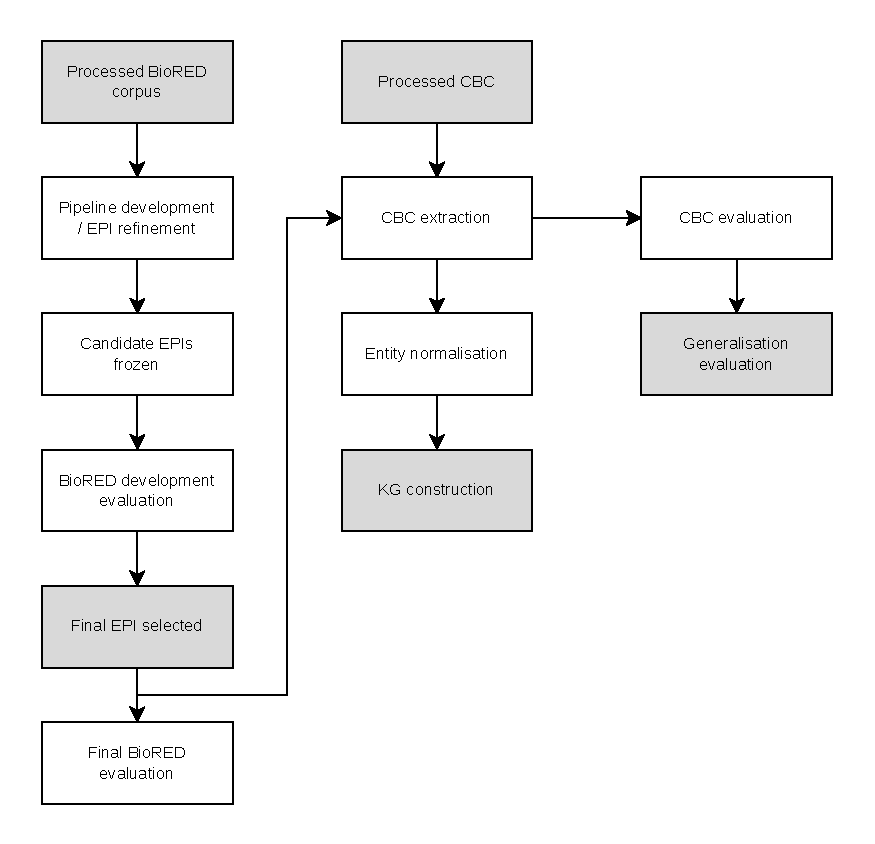
\includegraphics[width=\textwidth]{../img/system_architecture.pdf}
    \caption{System architecture and data flow, from prepared corpus input through extraction, normalisation, and \gls{kg} construction, to the three evaluation branches described in Section~\ref{sec:meth:evaluation}. Grey shading highlights key inputs, final stages, and outputs.}
    \label{fig:system_architecture}
\end{figure}

\section{Information Extraction Pipeline}
\label{sec:meth:info_extraction_pipeline}
Prepared title and abstract text produced in Section~\ref{subsec:meth:data_preparation}, was used as the input to a pretrained \gls{llm} accessed through an \gls{api}. \gls{ner} and \gls{re} were performed together within a single \gls{api} request per abstract, with the model instructed to return entities and relationships following the BioRED extraction schema. The raw response was parsed into structured entity and relation predictions and stored for subsequent evaluation and processing.

\subsection{LLM Configuration}
\label{subsec:meth:llm_config}
All extraction was performed using a single model, OpenAI's \verb|gpt-5.6-luna|, accessed via the OpenAI Python \gls{sdk}'s Responses \gls{api} (\verb|client.responses.create|). This pretrained model was used, without any parameter fine-tuning, across every \gls{epi} configuration, ensuring that any performance difference observed across \glspl{epi} resulted from changes to the pipeline's prompt and extraction setup rather than a change in the model's configuration. Higher-cost models, geared more towards complex reasoning over budget-consciousness, were considered for this project, such as \verb|gpt-5.6-sol| or \verb|gpt-5.6-sol|, however, they were deemed infeasible for this project given the number of \gls{api} calls required across iterative \gls{epi} development and the full extraction runs on all four splits: the BioRED training, development and test splits, and the full \gls{cbc}. No additional generation parameters were set for temperature or generation seed as \verb|gpt-5.6-luna| did not allow either as a tuneable parameter to any of their reasoning models.

\verb|gpt-5.6-luna|'s reasoning effort parameter (\verb|reasoning| $\in$ \{\verb|low|, \verb|high|, \verb|medium|\}), controlling the magnitude of internal reasoning before a response output, was also left at its default setting throughout this project, rather than being specifically tuned. Unlike model temperature, this was not a constraint of the model, but a deliberate choice made without deeper investigation into its effect on extraction quality and reasoning effort was not treated as a variable between \glspl{epi}. Increasing reasoning effort typically increases both time and cost demand per request, and investigating its effect on extraction precision, recall, and consistency was concluded to be out of the scope given the time and budget constraints discussed in Section~\ref{sec:meth:cost_analysis}. This parameter is one that a larger-budget project with longer timeframe allowance could reasonably investigate.

However, the absence of a temperature parameter and omission of fine-tuned reasoning parameter has a direct methodological consequence. Without these parameters, the model's output for a given prompt and abstract is not guaranteed to be identical across repeated calls, even when all else remains constant. This results in two distinct sub-consequences: firstly, as the reproducibility of an \gls{epi}'s outputs across multiple identical calls is not guaranteed, any \gls{epi} that reuses its previous \gls{epi}'s prompt reuses its stored outputs, rather than calling the model again. Secondly, an observed change in extraction performance between two \gls{epi}s using different prompt or extraction pipeline configurations cannot be attributed with complete certainty to the \gls{epi} refinement alone, as variation in performance may reflect natural variation in the model's generation, rather than just the effects of the update. This is partially mitigated by the fact that each \gls{epi} during the development stage was evaluated across the full BioRED training split ($n = 400$), rather than a small subsample of abstracts, which reduces the effects of variability of individual responses on performance metrics. Table \ref{tab:extraction_model_config_summary} summarises the chosen model's extraction pipeline configuration.

\begin{table}[H]
    \centering
    \caption{Extraction Model Configuration Summary}
    \label{tab:extraction_model_config_summary}
    \begin{tabularx}{\textwidth}{l l}
        \toprule
        Parameter & Value \\
        \midrule
        Model & \verb|gpt-5.6-luna| \\
        Provider / \gls{sdk} & OpenAI Python \gls{sdk}, Responses \gls{api} \\
        Fine-tuning & None \\
        Temperature & Default (not explicitly set) \\
        Reasoning & Default (not explicitly set) \\
        Maximum output tokens & Default (not explicitly set) \\
        Generation seed &  Default (not explicitly set) \\
        Request timeout & 120s \\
        Maximum automatic retries & 2 \\
        Same model used across all \glspl{epi} & Yes \\
        \bottomrule
    \end{tabularx}
\end{table}

\subsection{Prompt and Extraction Schema}
\label{subsec:meth:prompt_and_extraction_schema}
\gls{epi} configurations were stored in externally from the project's main Python code as a set of dictionaries in JSON format including the \gls{epi}'s name, prompt version --- also stored externally in a prompt configuration JSON file: rather than embedding text directly into the extraction code, evaluation version --- discussed in Section~\ref{subsec:meth:structured_output_and_parsing}, and additional notes.

The prompt used by the project's \glspl{epi} was structured around several main components: a task definition instructing the model to extract entities and relationships exactly as they would be annotated under the official BioRED annotation guidelines, the BioRED guidelines themselves \cite{luo2022_biored}, an explicit list of the allowed entity and relationship types, evidence requirements, few-shot examples, and explicit output format instructions specifying the required JSON output. Each prompt version sequentially introduced one or more new components, initialised with the baseline prompt, including only explicit general instructions of the extraction task and the structured JSON output.

The permitted entity and relation types instructed in the prompt corresponded exactly to BioRED's own schema, given in Table~\ref{tab:permitted_entity_and_relation_types}.

The official BioRED annotation guidelines \cite{luo2022_biored}, retrieved from the corpus's public GitHub repository in PDF form, provides information of the corpus's own construction that are not relevant to instructing an \gls{llm}'s extraction, such as the corpus's data sampling methodology, tools used in its ground truth construction, and its full reference list. Before incorporating the guidelines into the prompt, the document was therefore condensed to contain only the entity and relation annotation rules relevant to the extraction task itself. No semantic content within the filtered guidelines was altered --- only its structure was changed, converting the document's bullet formatting into a consistently headed, nested bullet-point structure intended to be more easily parsed by the \gls{llm} when called. This condensed guideline version was stored in \texttt{.txt} format and embedded directly into the prompt as \texttt{\{biored\_ext\_guidelines\}}. The complete filtered BioRED extraction guidelines are provided in Appendix~\ref{app:filtered_biored_guidelines}.

\begin{table}[H]
    \centering
    \caption{Permitted Entity and Relation Types}
    \label{tab:permitted_entity_and_relation_types}
    \begin{tabularx}{\textwidth}{l l}
        \toprule
        Entity types & Relation Types \\
        \midrule
        ChemicalEntity & Association \\
        DiseaseOrPhenotypic Feature & Bind \\
        GeneOrGeneProduct & Comparison \\
        SequenceVariant & Conversion \\
        OrganismTaxon & Cotreatment \\
        CellLine & Drug\_Interaction \\
         & Negative\_Correlation \\
         & Positive\_Correlation \\
        \bottomrule
    \end{tabularx}
\end{table}

The evidence requirements instructed the model to base extractions only on information explicitly supported by the given abstract to avoid inferring entities or relationships from background biomedical knowledge rather than the abstract text itself, to avoid treating multiple entity mentions in the same sentence or context as automatically associated, and to avoid inferring a more specific relation type such as \verb|Positive_Correlation| or \verb|Negative_Correlation| than what the text explicitly included. The model was also instructed to exclude a relationship where it was uncertain if it satisfied these criteria. For each entity, the model was required to return its text and entity type, and for each relationship triple, two entities and a relation type.

Few-shot examples constructed directly from BioRED's own training split ground truth annotations, with each example including an abstract's text and its correct entity and relationship annotations in the same JSON structure the model was instructed to output. Three constant few-shot examples were included in each prompt by default. Once generated in its first inclusion in a prompt, the few shot block was exported and stored for subsequent inclusion, sharing the same configuration, rather than being resampled on every execution.

\subsection{Structured Output and Parsing}
\label{subsec:meth:structured_output_and_parsing}
The \gls{llm} was instructed through the prompt to return its extractions as a single JSON object containing two top-level keys: \texttt{entities} and \texttt{relationships}, each a list of extractions. No \gls{api}-level constraint existed to enforce this structure, how closely the outputs adhered to the specified JSON output depended entirely on how well the model followed the prompt's explicit instructions.

Each abstract's raw response text was parsed as JSON in Python. Where a response failed to parse from JSON-structured string to valid JSON, this was recorded as a parse failure and the abstract was treated as having produced no entities and no relationships, rather than causing the run to fail. No further validation, such as checking that returned entity or relation types belonged to the allowed schema, was conducted beyond this JSON-validity check. Successfully parsed entities and relationships were converted into tuples following the form \texttt{(PMID, entity text, type)} for entities and \texttt{(PMID, entity 1, relation, entity 2)} for relationships. Entity text was stripped of any excess whitespace and stored in lowercase. These predictions sets were then converted into the same tabular structure used for BiORED's own ground-truth entities and relations, described in Section~\ref{subsec:meth:data_preparation}, allowing predicted and ground-truth extractions to be compared directly during evaluation.

Finally, after each \gls{epi}'s final extraction run on the entire BioRED train set, the run was exported as its own run in full, storing the \gls{epi}'s identifier (e.g.: \texttt{epi\_001}), the dataset split it was evaluated on, the prompt and evaluation version used, the number of abstracts processed, the count of failed JSON parses, the raw prompt template, each abstract's raw total model output, the parsed entity and relation predictions, and the evaluation metrics and errors resulting from that run. The raw and parsed extractions were stored as, as previously mentioned, when a new \gls{epi} reused the previous \gls{epi}'s prompt version and only updated the evaluation approach, the previous \gls{epi}'s outputs were used --- storing outputs allowed for the importing of previous \gls{epi} outputs when necessary. How these logged runs were compared and used to select a final \gls{epi} is described in Section~\ref{sec:meth:pipeline_development}. The complete text of each prompt version is provided in Appendix~\ref{app:extraction_prompts}.

\section{Pipeline Development}
\label{sec:meth:pipeline_development}
Development of the extraction pipeline was organised as a sequence of Extraction Pipeline Iterations \glspl{epi}. Each \gls{epi} represented a pre-configured combination of a prompt version and evaluation version and was assigned a unique identifier (e.g., \texttt{epi\_001}) used to track it during development. Changes between \glspl{epi} were introduced incrementally, with each new \gls{epi} modifying one or a few components of the previous iteration, so that the effect of an individual methodological change could be isolated, rather than observing the effects of several significant changes. As described in Section~\ref{sec:meth:research_design}, all \gls{epi} development and refinement was conducted exclusively against the BioRED training split, with the BioRED development split used for the comparison of candidate \glspl{epi}, playing no role in extraction pipeline refinement. Each \gls{epi}'s full configuration, prompt template, and extraction outputs were automatically logged after extraction, allowing outputs to be reused directly by a subsequent \gls{epi} where prompt version remained unchanged between them.

\subsection{Extraction Pipeline Iterations}
\label{subsec:meth:extraction_pipeline_iterations}
Table~\ref{tab:epi_summary} summarises the configuration of all \glspl{epi} produced during development, including the main methodological change in addition to the previous iteration.

\begin{table}[H]
    \centering
    \caption{Extraction Pipeline Iteration summary}
    \label{tab:epi_summary}
    \begin{tabularx}{\textwidth}{@{} l p{2.4cm} p{4.0cm} X @{}}
        \toprule
        EPI & Prompt & Evaluation & Main addition/purpose \\
        \midrule
        \texttt{epi\_001} & \texttt{v1} & \texttt{v1} (strict matching) & Baseline configuration \\
        \texttt{epi\_002} & \texttt{v1} & \texttt{v2} (relaxed matching) & Relaxed matching to baseline prompt \\
        \texttt{epi\_003} & \texttt{v2} & \texttt{v2} & Filtered BioRED guidelines and allowed entity and relation types \\
        \texttt{epi\_004} & \texttt{v2} & \texttt{v3} (cosine matching) & Cosine matching \\
        \texttt{epi\_005} & \texttt{v3} & \texttt{v3} (cosine matching) & Few-shot examples \\
        \texttt{epi\_006} & \texttt{v3} & \texttt{v4} (relation order invariance) & Relation order invariant evaluation \\
        \texttt{epi\_007} & \texttt{v4} & \texttt{v4} & Targeted suppression of background biomedical knowledge \\
        \texttt{epi\_008} & \texttt{v5} & \texttt{v4} & Explicit instructions preventing inference of an unsupported extraction \\
        \texttt{epi\_009} & \texttt{v6} & \texttt{v4} & Explicit precision-over-recall instructions \\
        \texttt{epi\_010} & \texttt{v7} & \texttt{v4} & Precision-focussed conservative extraction instructions \\
        \texttt{epi\_011} & \texttt{v8} & \texttt{v4} & Targeted suppression of excessive relation over-extraction \\
        \bottomrule
    \end{tabularx}
\end{table}

Together, this sequence of pipeline iterations reflects several broad stages of development, rather than a linear progression of independent changes: an initial baseline extraction stage (\texttt{epi\_001}-\texttt{002}), alignment of the prompt with BioRED's own entity and relation schema (\texttt{epi\_003}-\texttt{004}), introduction of few-shot prompting (\texttt{epi\_005}), concurrent evaluation logic progression (\texttt{epi\_001}--\texttt{006}), tightening of evidence requirements (\texttt{epi\_007}--\texttt{008}), and a final stage of prompt refinement targeting over-extraction (\texttt{epi\_009}--\texttt{011}). It should be noted that, for each \gls{epi} where evaluation methodology was updated, the previous \gls{epi}'s prompt outputs were used. This allowed direct analysis of the evaluation refinement's effects on extraction performance metrics.

As mentioned above, evaluation methodology applied to each \gls{epi}'s outputs also evolve over the course of development, concurrently with prompt refinement. As summarised in Table~\ref{tab:epi_summary}, the baseline \gls{epi} was assessed using strict matching, where only exact string matching between an extraction and a ground-truth counted as a success. Manual inspection of errors --- automatically recorded in each \gls{epi}'s stored log, including \glspl{fp} and \glspl{fn} --- indicated that numerous extractions represented the correct biomedical concept, yet differed from the ground-truth annotation in span boundary or string representation, meaning strict matching classified some semantically correct predictions as errors. This motivated the introduction of relaxed matching, which allowed correct-match classification where the string representation of the extracted entity differed slightly from that of its corresponding ground truth. However, this implementation was found to be insufficient where an extraction and its ground truth were semantically equivalent but expressed using disparate string representations, exceeding solely a mismatch between entity name boundaries. As a result, subsequent cosine-similarity-based matching was introduced, which compared the vector embeddings of extracted and ground truth entity mentions using a fixed threshold. The exact configuration and implementation of strict, relaxed, cosine, and relation order invariance evaluation approaches are described in Section~\ref{sec:meth:evaluation}.

% Put in Sec. 4.7
% Embeddings were generated using \texttt{S-PubMedBert-MS-MARCO} \pref, a Sentence-BERT model pretrained on PubMed abstracts and fined tuned for semantic search on the Microsoft Machine Reading Comprehension (MS MARCO) dataset. This model was selected over general-purpose alternatives, such as OpenAI's \texttt{text-embedding-3-large}, as the fine-tuned, domain specific model was expected to produce more accurate representations of biomedical terminology, where subtle differences between distinct concepts are captured, where general-purpose embedding models are not trained to.

% For each extraction--ground truth comparison, cosine similarity was computed between embedding vectors, and a match was recorded where this similarity met or exceeded a pre-defined threshold of 0.85. Matching was performed in a greedy approach, where for each predicted mention, the highest-scoring unmatched ground truth mention was selected as a match and removed from evaluation of subsequent extractions. This prevented evaluation where a single ground truth annotation counted as a match for multiple extractions.

% Include strict, relaxed, and how relation order invariance applies to all evaluation methods for relations

% After analysis of initial cosine evaluation implemented in \texttt{epi\_005}'s extraction performance, errors indicated that a few relation extractions were marked as non-matches where the extracted relation's entities appeared in the opposite order of their corresponding ground truth. As a result, relation order invariance matching was introduced where both orders of a relationship triple's entities were evaluated, where a match of either order counted as a correct extraction for that extraction--ground truth pair:

% \vspace{0.75em}
% \newcommand{\triple}[3]{(\text{#1},\, \text{#2},\, \text{#3})}

% \noindent\textbf{Before relation order invariance:}
% \vspace{0.25em}
% \[
% \triple{warfarin}{Positive\_Correlation}{ICH}
% \;\neq\;
% \triple{ICH}{Positive\_Correlation}{warfarin}
% \]

% \noindent\textbf{After relation order invariance:}
% \vspace{0.25em}
% \[
% \triple{warfarin}{Positive\_Correlation}{ICH}
% \;\equiv\;
% \triple{ICH}{Positive\_Correlation}{warfarin}
% \]

When necessary, to understand the nature of extraction errors, false positive (\gls{fp}) and false negative (\gls{fn}) relation errors produced by the current \gls{epi} were sampled and analysed. This analysis was restricted to relations, rather than entities, as relation extraction exhibited significantly weaker performance throughout development and was therefore the main focus of this investigation. For the selected \gls{epi}, up to 50 false positive \gls{fp} and 50 false negative \gls{fn} errors were randomly sampled, using a fixed random seed for reproducibility, and assigned one of a set of pre-defined error categories.

Given the volume of errors sampled, manual assignment of each error to a pre-defined error category was not feasible. Instead, categorisation was performed automatically using the same \gls{llm} used for the extraction process. For each sampled error, the model was provided with the incorrect relation, the error type (\gls{fn} or \gls{fp}), the source abstract, and the corresponding BioRED ground truth relations for that abstract. The model was then instructed to assign the error to exactly one of seven predefined error categories (Table~\ref{tab:error_categories}), each including a description of the conditions of when the error category is true. The complete prompt supplied to the \gls{llm} during error analysis is provided in Appendix~\ref{app:sec:error_categorisation_prompt}.

\begin{table}[H]
    \centering
    \caption{Error category summary}
    \label{tab:error_categories}
    \begin{tabularx}{\textwidth}{l X}
        \toprule
        Category & Description \\
        \midrule
        Wrong relation type & "The correct entity pair is identified, but the predicted relation type differs from the BioRED ground truth." \\
        Duplicate/coreference & "The error results from duplicate entity mentions, abbreviations, aliases, or coreferential mentions of the same underlying entity." \\
        Unsupported relation & "The predicted relation is not supported by the abstract or BioRED annotation policy." \\
        Entity boundary/synonyms mismatch & "The prediction and ground truth refer to the same underlying entity, but differ in span, wording, abbreviation, or synonym representation." \\
        Missing relation & "A BioRED ground-truth relation is supported by the abstract but was not extracted by the system." \\
        Evaluation artefact & "The prediction is substantively compatible with the ground truth, but is counted as an error because of the evaluation or matching procedure." \\
        Other/unclear & "The primary cause cannot be confidently assigned to any other category." \\
        \bottomrule
    \end{tabularx}
\end{table}

These category distributions were used diagnostically, precision, recall, and F1 to establish whether an \gls{epi}'s performance reflected true extraction failure, evaluation artefacts, or specific prompt configuration issues. Analysis showed that unsupported relations was a significant false-positive category through much of development, directly motivating the evidence requirement prompt refinements in \texttt{epi\_007}--\texttt{epi\_011}. A significant proportion of false negatives were also categorised as evaluation artefacts, supporting the introduction of cosine-based matching. Figure~\ref{fig:epi_003_train_error_distribution} shows a representative error distribution figure from one stage of this analysis (\text{epi\_009}) --- the remaining error distribution figures are shown in Appendix~\ref{app:epi_error_dist_figures}.

\begin{figure}[H]
    \centering
    
\includegraphics[width=1\textwidth]{../../../img/error_analysis/biored_train/epi_009.png}
    \caption{\texttt{epi\_003} relation error distribution.}
    \label{fig:epi_003_train_error_distribution}
\end{figure}

\subsection{Development and Model Selection}
\label{subsec:meth:development_and_model_selection}
Iterative \gls{epi} development against the BioRED training split contiued until further prompt or evaluation refinements produced only marginal changes in extraction performance metrics. At this point, all candidate \gls{epi} configurations were frozen and no further prompt or schema adjustment was made

Figure~\ref{fig:epi_performance} in Section~\pref \ shows the entity and relation precision, recall, and F1 across all \glspl{epi} measured on the BioRED development split, after being refined on the training split, allowing performance to be tracked across sequential extraction pipeline refinements. On the basis of primarily F1, and secondarily precision and recall, \texttt{epi\_007}, \texttt{epi\_008}, and \texttt{epi\_009} were selected for further comparison.

Figure~\ref{fig:top3_epi_relation_performance} (Section~\pref) compares these three selected \glspl{epi} directly on relation precision, recall, and F1, again, evaluated on the unseen BioRED development split. Final selection between the three candidates was mainly based on relation F1, as relation extraction was the main target of refinement at this stage of development. \texttt{epi\_009} was selected as it exhibited the highest F1 and precision, while narrowly underperforming compared to \texttt{epi\_007} on recall. It should be noted that while \texttt{epi\_009} marginally outperformed its competitors on balance, the differences in extraction performance for all three performance metrics were near negligible.

No further prompt, schema, or evaluation changes were made to the selected \gls{epi} following this comparison. The resulting configuration was therefore frozen and used without modification for the final BioRED benchmark evaluation and extraction of the \gls{cbc}.

\subsection{Final Pipeline}
\label{subsec:meth:final_pipeline}
The final extraction pipeline configuration selected through the process above is summarised in Table~\ref{tab:final_epi_config}

\begin{table}[H]
    \centering
    \caption{Final Extraction Pipeline Configuration}
    \label{tab:final_epi_config}
    \begin{tabularx}{\textwidth}{l X}
        \toprule
        Component & Final configuration \\
        \midrule
        \gls{epi} & \texttt{epi\_009} \\
        Prompt version & \texttt{v6} (Suppression of background knowledge, unsupported extraction inference suppression) \\
        Evaluation version & \texttt{v4} (Cosine-based, relation order invariant) \\
        \gls{llm} & \texttt{gpt-5.6-luna} \\
        Few-shot examples & 3 fixed BioRED training examples \\
        Entity schema & BioRED six entity types (Table~\ref{tab:permitted_entity_and_relation_types}) \\
        Relation schema & BioRED eight relation types (Table~\ref{tab:permitted_entity_and_relation_types}) \\
        Output format & JSON object \\
        \bottomrule
    \end{tabularx}
\end{table}

\section{Contemporary Knowledge Graph Construction}
\label{sec:meth:contemporary_kg_construction}

\subsection{Contemporary Corpus Extraction}
\label{subsec:meth:contemporary_corpus_extraction}

\subsection{Graph Construction}
\label{subsec:meth:graph_construction}

\subsection{Ontology-Based Validation}
\label{subsec:meth:ontology_based_validation}

\section{Evaluation}
\label{sec:meth:evaluation}

\subsection{Entity Evaluation}
\label{subsec:meth:entity_evaluation}

\subsection{Relation Evaluation}
\label{subsec:meth:relation_evaluation}

\subsection{Generalisation Evaluation}
\label{subsec:meth:generalisation_evaluation}

\subsection{Knowledge Graph Evaluation}
\label{subsec:meth:knowledge_graph_evaluation}

\section{Cost Analysis}
\label{sec:meth:cost_analysis}

\chapter{Results}
\begin{table}[H]
    \centering
    \caption{Entity Extraction Performance}
    \label{tab:entity_results}
    \begin{tabularx}{\textwidth}{l l r r r}
        \toprule
        EPI & Reported matching approach & Precision & Recall & F1 \\
        \midrule
        \texttt{epi\_001} & Strict & 0 & 0 & 0 \\
        \texttt{epi\_002} & Relaxed & 0 & 0 & 0 \\
        \texttt{epi\_003} & Relaxed & 0.865 & 0.774 & 0.817 \\
        \texttt{epi\_004} & Cosine & 0.894 & 0.800 & 0.845 \\
        \texttt{epi\_005} & Cosine & 0.930 & 0.736 & 0.821 \\
        \texttt{epi\_006} & Cosine + relation order invariance & 0.930 & 0.736 & 0.821 \\
        \texttt{epi\_007} & Cosine + relation order invariance & 0.918 & 0.762 & 0.833 \\
        \texttt{epi\_008} & Cosine + relation order invariance & 0.901 & 0.765 & 0.828 \\
        \texttt{epi\_009} & Cosine + relation order invariance & 0.935 & 0.761 & 0.839 \\
        \texttt{epi\_010} & Cosine + relation order invariance & 0.941 & 0.754 & 0.837 \\
        \texttt{epi\_011} & Cosine + relation order invariance & 0.932 & 0.738 & 0.824 \\
        \bottomrule
    \end{tabularx}
\end{table}

\begin{table}[H]
    \centering
    \caption{Relation Extraction Performance}
    \label{tab:relation_results}
    \begin{tabularx}{\textwidth}{l l r r r}
        \toprule
        EPI & Reported matching approach & Precision & Recall & F1 \\
        \midrule
        \texttt{epi\_001} & Strict & 0 & 0 & 0 \\
        \texttt{epi\_002} & Relaxed & 0 & 0 & 0 \\
        \texttt{epi\_003} & Relaxed & 0.192 & 0.189 & 0.190 \\
        \texttt{epi\_004} & Cosine & 0.423 & 0.416 & 0.420 \\
        \texttt{epi\_005} & Cosine & 0.392 & 0.419 & 0.405 \\
        \texttt{epi\_006} & Cosine + relation order invariance & 0.478 & 0.511 & 0.494 \\
        \texttt{epi\_007} & Cosine + relation order invariance & 0.495 & 0.524 & 0.509 \\
        \texttt{epi\_008} & Cosine + relation order invariance & 0.487 & 0.516 & 0.501 \\
        \texttt{epi\_009} & Cosine + relation order invariance & 0.502 & 0.516 & 0.509 \\
        \texttt{epi\_010} & Cosine + relation order invariance & 0.501 & 0.488 & 0.494 \\
        \texttt{epi\_011} & Cosine + relation order invariance & 0.501 & 0.456 & 0.478 \\
        \bottomrule
    \end{tabularx}
\end{table}

\begin{figure}[H]
    \centering
    
\includegraphics[width=1\textwidth]{../../../img/dev_analysis/epi_performance.png}
    \caption{EPI Performance}
    \label{fig:epi_performance}
\end{figure}

\begin{figure}[H]
    \centering
    
\includegraphics[width=1\textwidth]{../../../img/dev_analysis/top3_relation_f1.png}
    \caption{Selected three best-performing \glspl{epi}}
    \label{fig:top3_epi_relation_performance}
\end{figure}

\begin{figure}[H]
    \centering
    
\includegraphics[width=1\textwidth]{../../../img/generalisation_evaluation/entity_generalisation.png}
    \caption{Entity Generalisation: BioRED vs. CBC}
    \label{fig:entity_generalisation}
\end{figure}

\begin{figure}[H]
    \centering
    
\includegraphics[width=1\textwidth]{../../../img/generalisation_evaluation/relation_generalisation.png}
    \caption{Relation Generalisation: BioRED vs. CBC}
    \label{fig:relation_generalisation}
\end{figure}
\include{chapters/06_discussion}
\include{chapters/07_conclusion}

\bibliographystyle{unsrt}
\bibliography{bibliography}

\appendix

\chapter{Filtered BioRED Annotation Guidelines Used For Prompting}
\label{app:filtered_biored_guidelines}
\begin{lstlisting}
## Guideline of the entities

### General rules
- Annotate all the spans of all the six concept types.
- The full text can be accessed to clarify the concept spans and identifiers.
- The abbreviation and its long form should be annotated separately if possible. prostaglandin E2 (PGE2) in the text, "prostaglandin E2" and "PGE2" should be both annotated to chemicals with the same identifier (D015232).
- Annotate both the full name and abbreviation in one entity, if the boundary of the entity covers both of them. For instance, annotate "Deoxyguanosine kinase (dGK) deficiency" entirely to a disease (PMID:19394258).
- Annotate the composite entity spans (e.g., "MMP-1, -2") entirely. The identifiers of the multiple concepts should
be entered separated by "," with no space (e.g., "4312,4313").
- Annotate any concept identifier span (e.g., "OMIM 307800" and "rs729302").
- Annotate the concept spans with misspelling ("HLRRC" in PMID:18366737).

### Gene
- The gene spans should be linked to NCBI Gene ID (https://www.ncbi.nlm.nih.gov/gene/). Specify the corresponding species and the identifiers to the gene spans.
- Annotate the gene families including paralogs/orthologs (e.g., bone morphogenetic protein(bmp)), but DO NOT annotate the functional based families (e.g., tumor suppressor gene, protein kinase).
- Following the previous rule, if at least one of the gene family members mentioned in the text, the identifiers of those members are assigned to the family name (e.g., in "Cytochrome P-450 genes (CYP1A1, CYP2A6, CYP2D6, and CYP2E1)", Cytochrome P-450 genes should be assigned with NCBI Gene: 1543,1548,1565,1571). If no family member is in the text, the first gene reached in the gene family should be assigned (e.g., matrix metalloproteinases to NCBI Gene:4312(MMP1)).
- In experimental studies, annotate the gene identifier corresponding to the organism/species that is the source of the
gene (for example mouse gene transfected into human cells is annotated to record for mouse gene).
- DO NOT annotate the genes, if they are named for cells and pathways.

### Disease
- The diseases refer to MEDIC which is a combination of MESH (https://meshb.nlm.nih.gov/search) and OMIM (https://omim.org/). We annotate the MESH identifier, if a disease has both the MESH and OMIM identifiers.
- If no specific disease concept can be reached in MEDIC by the annotated span, we annotate the closest hypernym concept that logically describes the disease span(e.g., X-linked retinitis pigmentosa to D012174 (retinitis pigmentosa) in PMID:17935240). Otherwise, "-" is assigned to the mismatched diseases.
- Annotate the diseased-related phenotypes but not other (e.g., short ear in PMID:17345627).
- DO NOT annotate the high-level diseases (e.g., "genetic disorder").
Excludes:
- Cis-acting disease (PMID:12442272)
- genetic disorders (PMID:18046082)
- familial disorder (PMID:20806042)
- Annotate "drug addiction" to "disease".
- Annotate the symptoms to diseases.
- DO NOT annotate overdose.
- DO NOT annotate the mental status and phenotypes to diseases unless the term is exactly recorded in MEDIC. e.g., decline in sympathetic tone (PMID:19067809)
- DO NOT annotate references to biological processes such as "tumorigenesis" or "cancerogenesis".
- Annotate minimum necessary text spans for a disease. For example, select "hypertension" instead of "sustained hypertension.", unless the span covers the prefix or the suffix can exactly match a specific concept identifier (e.g., "chronic bronchitis" to D029481).

### Chemical
- Chemical spans should be linked to MESH (https://meshb.nlm.nih.gov/search). "-" is assigned to the mismatched chemicals.
- Annotate the chemical abbreviation with the dose. For example "In addition, GABA content of mice hippocampus treated with GFC75 plus P400 showed an increase of 46.90% when compared with seized mice.", 75 and 400 suffixes are the doses. In this case, we annotate GFC75 and P400 as chemical spans. (PMID:24911645).
- Annotate the chemical resource for extracts, e.g., "ethanolic extract of Daucus carota seeds (DCE)" in PMID:16755009; "grape seed proanthocyanidin extract" in PMID:11334364.
- DO NOT annotate antibodies to chemicals. (PMID:17595233) (PMID:20648600)
- DO NOT annotate saline, placebo, water, and juice.
- DO NOT annotate residue, free radicals.
- DO NOT annotate staining chemical (e.g., hematoxylin in PMID:24442316)
- DO NOT annotate vaccines.

### Species
- The species spans should be linked to NCBI Taxonomy ID (https://www.ncbi.nlm.nih.gov/taxonomy/)
- DO NOT annotate beyond species rank (e.g., annotate homo sapiens but do not annotate mammalian which is a taxonomy class)

### Variant
- The annotation of the variants follows tmVar annotation guidelines, the variants should be linked to dbSNP (https://www.ncbi.nlm.nih.gov/snp) accession number (RS#) when possible. Otherwise, we annotate the variant components (e.g., wild type, location, and mutant) following the tmVar component format (e.g., V600E to "p|SUB|V|600|E").
- DO NOT annotate residue of the gene modification.
- For those variants that cannot be normalized: In our observations on the variant recognition/normalization dataset, around 50-60% of the variants cannot be normalized to the specific concept identifiers in dbSNP. For those, we enumerate the components of the variants.

### Normalized components of the curated variant types:

#### Variant on DNA Sequence
Example(s) and normalized component or identifier(s):
- c.1922G>A: c|SUB|G|1922|A
- C-to-G transition was identified at nucleotide 857: c|SUB|C|857|G

#### Variant on protein sequence
Example(s) and normalized component or identifier(s):
- R114H: p|SUB|R|114|H
- methionine to threonine substitution at codon 235: p|SUB|M|235|T

#### RS number
Example(s) and normalized component or identifier(s):
- rs763780: rs763780

#### Allele on DNA sequence
Example(s) and normalized component or identifier(s):
- -281G: c|Allele|G|-218

#### Allele on protein sequence
Example(s) and normalized component or identifier(s):
- L638: p|Allele|L|638
- stop codon at position 372: p|Allele|X|372

#### Nucleotide or acid change
Example(s) and normalized component or identifier(s):
- G > C: c|SUB|G||C
- valine for glutamate: p|SUB|V||E

## Guideline of the relation pairs

### General rules
- We only annotate the (1) Popular associations and the (2) Corresponding gene/species in Figure 1.
- Co-occurrence in the same sentence is not required.
- DO NOT annotate a confirmed irrelevance. (e.g., "Nonetheless, NBS1 gene heterozygosity is not a major risk
factor for lymphoid malignancies in childhood and adolescence" in PMID:16152606)
- Annotate the associations with explicit statements in the text.
- The full text is NOT allowed to access. DO NOT annotate if the statement in the abstract is not clear. (e.g.,
PMID:14722929)
- For Co-treatment, we annotate "Negative_Correlation" between the two chemicals and the disease, and a
"Cotreatment" relation between the two chemicals. For an example in PMID:16720068, "Possible neuroleptic
malignant syndrome related to concomitant treatment with paroxetine and alprazolam.".
- For Drug_Interaction, we annotate "Positive_Correlation" between the two chemicals and the disease, and a
"Drug_Interaction" relation between the two chemicals.

### Disease-chemical
- Annotate the association of chemicals and disease due to the "toxicity" and "drug-induced", but not annotate the
chemicals with the disease concept-"toxicity" directly.
    -  PMID:19728177
    "RESULTS: Our patient was admitted to the MICU after being found unresponsive with presumed toxicity from acetaminophen which was ingested over a 2-day period. ... In patients with FHF and cerebral edema from acetaminophen overdose, prolonged therapeutic hypothermia could potentially be used as a life saving therapy and a bridge to hepatic and neurological recovery." We annotate the associations between acetaminophen and FHF/cerebral edema due to the toxicity, but we do not annotate acetaminophen and toxicity.
- Annotate the relation between the target disease and the measure level of the molecules/chemicals in blood test
with correlation, "Compared with control patients, CRF and ESRD patients had higher preoperative serum
creatinine levels, a greater percentage of patients with hepatorenal syndrome.", the pairs of "CRF, creatinine" and
"ESRD, creatinine" is annotated. (PMID:11773892)
- DO NOT annotate the association of disease to the staining chemicals. For instance, "The extent of neuronal injury
was determined by 2,3,5-triphenyltetrazolium staining." (PMID:1711760) and "Renal lesions were analyzed in
hematoxylin and eosin, periodic acid-Schiff, and Masson's trichrome stains. SRL-treated rats presented proteinuria
and NGAL (serum and urinary) as the best" (PMID:24971338)
- DO NOT annotate the association of any disease with the chemical concept "analgesia" in "patient-controlled
analgesia (PCA) pump". For instance, "patient-controlled analgesia (PCA) pump" (PMID:9672936)
- DO NOT annotate toxicity with its chemical. For instance, do not annotate "unresponsive with presumed toxicity
from acetaminophen" (PMID:19728177)
- Annotate the chemicals which prevents the chemical-induced disease (PMID:24971338+18503483)

### Disease-gene
- DO NOT annotate the prognostic factor of genes or its variants to the target disease.
- Annotate the negative correlation (e.g., knockdown gene to the target disease). For instance, annotates Gankyrin
and HCC in "Gankyrin expression in the tumor microenvironment is negatively correlated with progression-free
survival in patients undergoing sorafenib treatment for HCC." (PMID:28777492)
- DO NOT annotate the symptoms of the target disease to the correlated variants or genes, unless the clear statement
between the symptom and variant is provided.

### Disease-variant & Disease-gene
- Annotate the corresponding diseases with the variant when it is observed in patients.
- Annotate the diseases with the associated genes.
- Annotate the corresponding gene of the variant with the variant-associated disease.
- Annotate the association between the variants (and corresponding gene) and the diseases belonging to the target
disease. For instance, annotate the association between "autosomal recessive disease" and "272gly----stop"
(PMID:1671881).
- Annotate the minor association (e.g., the observation of the association on few patients).
- Annotate the associations in the particular races.
- Annotate the association between disease and variant if the inheritance of the genetic disease is confirmed by the
variant.
- DO NOT annotate the symptoms of the target disease to the correlated variants or genes, unless the clear statement
between the symptom and variant is provided. (ex in PMID: 1952108)

### Gene-gene
- Annotate the pairs of the members in the protein complex, e.g., EPO/EPOR (PMID:22808010).
    - In "We cloned the cDNA of three remaining human NADH:ubiquinone oxidoreductase subunits of this IP fraction: the NDUFS2 (49 kDa), NDUFS3 (30 kDa), and NDUFS6 (13 kDa) subunits.", all the pairs between two of the NDUFS2, NDUFS3, and NDUFS6 are annotated. (PMID:9647766)
- DO NOT annotate the "is_a" association between two genes. For instance, DO NOT annotate "breast and ovarian
cancer gene" and "BRCA1" (PMID:8944024).
- Annotate protein-protein interaction for singling proteins and the receptors. For instance, "Epo-R signaling
proteins (Akt, STAT5, p70s6k, LYN, and p38MAPK)" (PMID:27640183)

### Gene-chemical
- Annotate the chemical with the gene receptor. For instance, "antipsychotic drugs that have a high affinity with the
D2 receptor" (PMID:16867246)

### Chemical-chemical
- DO NOT annotate the "is_a" association between two chemicals. For instance, "Nefiracetam is a novel
pyrrolidone derivative" (PMID:8829135)
- Annotate the chemical-chemical association for the chemical contributes to the other for treatment, side effects and
drug-drug interaction. In "the midline serotonin B3 cells in the medulla contribute to the hypotensive action of
methyldopa", the pair of serotonin and methyldopa is annotated. (PMID:2422478)

### Chemical-variant
- Annotate the chemical with the variant, if the chemical binding ability of the gene impaired by the variant. For
instance, "This variant (apoE Guangzhou) may cause a marked molecular conformational change of the apoE and
thus impair its binding ability to lipids." (PMID:18046082)
- Annotate the chemical with the variant, if different mRNA stability between different alleles affected by the
chemical. For instance, "After transfection and inhibition of transcription with actinomycin D, analysis of mRNA
turnover failed to reveal differences in mRNA stability between A118 and G118 alleles, indicating a defect in
transcription or mRNA maturation." (PMID:16046395)

### Others
- DO NOT annotate the pairs of concepts with negative conclusions (e.g., "not significant", "no correlation was
observed"). For instance, "For most of the variants identified in the Kenyan and Sudanese study population, a
causative association with NSARD appears to be unlikely" is not annotated.
- In the case that a disease is induced by a chemical, and the other concepts (e.g., chemical, or protein) treats/affects
the induced disease, we annotate the three pairs by following examples. For instance:
    -  "In addition, there is convincing clinical evidence that monotherapy with continuous subcutaneous apomorphine infusions is associated with marked reductions of preexisting levodopa-induced dyskinesias." (PMID:11009181)
        - Positive_Correlation between levodopa and dyskinesias
        - Negative_Correlation between apomorphine and dyskinesias
        - Negative_Correlation between apomorphine and levodopa
    - Absence of PKC-alpha attenuates lithium-induced nephrogenic diabetes insipidus. (PMID:25006961)
        - Positive_Correlation between lithiumand nephrogenic diabetes
        - Positive_Correlation between PKC-alpha and dyskinesias
        - Positive_Correlation between PKC-alpha and lithium
    - Characterization of a novel BCHE "silent" allele: point mutation (p.Val204Asp) causes loss of activity and prolonged apnea with suxamethonium. (PMID:25054547)
        - Positive_Correlation between p.Val204Asp and apnea
        - Negative_Correlation between apnea and suxamethonium
        - Association between p.Val204Asp and suxamethonium
        - Association between BCHE and apnea
        - Association between BCHE and suxamethonium
    -  Curcumin prevents maleate-induced nephrotoxicity (PMID:25119790)
        - Negative_Correlation between Curcumin and nephrotoxicity
        - Positive_Correlation between maleate and nephrotoxicity
        - Negative_Correlation between Curcumin and maleate
- Annotate the previous reported association, even the conclusion demonstrates the association is not significant. (PMID:15824163)

### Guideline of the relation types
We collected a list of relation types between two concepts (e.g., upregulation between two genes). Further, we merged some of the relation types to narrow down the curation complexity and increase the number of instances in each relation type.

The following mappings define how directional relation types should be converted to the BioRED relation types.
**Gene <-> Gene**
| Directional relation | BioRED relation |
|----------------------|-----------------|
| Upregulation | Positive_Correlation |
| Downregulation | Negative_Correlation |
| Regulation | Association |
| Positive_Correlation | Positive_Correlation |
| Negative_Correlation | Negative_Correlation |
| Bind | Bind |
| Modification | Association |
| Association | Association |

**Chemical <-> Gene**
| Directional relation | BioRED relation |
|----------------------|-----------------|
| Exhibition (Chemical -> Gene) | Positive_Correlation |
| Response (Gene -> Chemical) | Positive_Correlation |
| Suppression (Chemical -> Gene) | Negative_Correlation |
| Resistance (Gene -> Chemical) | Negative_Correlation |
| Association | Association |
| Receptor | Bind |
| Chem_Modification | Association |

**Chemical <-> Variant**
| Directional relation | BioRED relation |
|----------------------|-----------------|
| Association | Association |
| Resistance | Negative_Correlation |
| Response (and sensitivity) | Positive_Correlation |

**Gene <-> Disease**
| Directional relation | BioRED relation |
|----------------------|-----------------|
| Positive_Correlation | Positive_Correlation |
| Negative_Correlation | Negative_Correlation |
| Association | Association |

**Variant <-> Disease**
| Directional relation | BioRED relation |
|----------------------|-----------------|
| Cause | Cause |
| Association | Association |

**Chemical <-> Disease**
| Directional relation | BioRED relation |
|----------------------|-----------------|
| Treatment | Negative_Correlation |
| Induce | Positive_Correlation |
| Association | Association |

**Chemical <-> Chemical**
| Directional relation | BioRED relation |
|----------------------|-----------------|
| Cotreatment | Cotreatment |
| Inhibition | Negative_Correlation |
| Increase | Positive_Correlation |
| Drug_Interaction | Drug_Interaction |
| Association | Association |
| Comparison | Comparison |

### Disease-chemical
- Positive_Correlation
    - Chemical-induced disease.
    - Chemical (or Higher dose of the chemical) causes a higher risk of the disease.
    - Disease causes the increase of the chemical measured level.
    - The level of the chemical and the risk of the disease present a positive correlation.
    - Chemical exposures during development alter disease susceptibility later in life.
- Negative_Correlation
    - The disease-treated chemical/drug.
    - Disease causes the decrease of the chemical measured level.
    - The chemical/drug drops down the susceptibility of the disease.
- Association
    - A safety drug of the potential disease (PMID:20722491 - capecitabine(C110904) - hepatic and renal dysfunctions(D008107|D007674))
    - The associations of the pairs which cannot be categorized to positive/negative correlation.
    - The associations without clear description.

### Disease-gene
- If an association between a variant and a disease is confirmed, the corresponding gene should associate with the disease by "Association" type.
- Positive_Correlation
    - The overdose of protein causes the disease.
    - The knockout gene prevents the disease.
    - The side effect of protein (drug) causes the disease
- Negative_Correlation
    - The protein (drug) is used to treat/prevent the disease.
    - Lack of the protein causes the disease.
    - The knockout gene causes the disease.
- Association
    - The associations of the pairs which cannot be categorized to previous relation types.
    - The associations without clear description.
    - The functional gene prevents the occurrence of the disease.
    - Protein deficiency.

### Disease-variant
- Positive_Correlation
    - The variant increases the risk of the disease.
    - Significant frequency (p-value) of the disease with the specific allele.
    - The variant causes the gene to be either over-express or non-functional and further causes disease (or raises the disease susceptibility).
    - Disease is caused by protein deficiency, and the variant is responsible for the deficiency.
    - The variant plays a role in genetic predisposition to the disease.
    - The variant has a significant contribution to the disease.
    - Annotate "Positive_Correlation" to the pair of "founder mutation" and the target disease. (PMID:10788334,19394258)
- Negative_Correlation
    - The variant decreases the risk of the disease.
- Association
    - The variant observed from a number of patients.
    - The variant is associated with a lower prevalence of the disease or is responsible for the lower disease susceptibility
    - The associations of the pairs which cannot be categorized to "Cause" relation type.
    - The associations without clear description.
### Gene-gene
- Positive_Correlation
    - Two genes present the positive correlation in gene expression results.
    - Gene A is a transcription factor of the gene B, and gene A upper regulates the gene B.
    - Two genes present a positive correlation in any way.
- Negative_Correlation
    - Two genes present the negative correlation in gene expression results.
    - Gene A is a transcription factor of the gene B, and gene A down regulates the gene B.
    - Two genes present a negative correlation in any way.
- Bind
    - physical interaction between two proteins.
    - Protein A binds the promoter of gene B.
    - Two or more proteins in a complex.
    - Annotate "bind" to the protein and its protein receptor. ("androgen receptor" and "androgen" in PMID:15599941)
    - If the binding causes a positive or negative correlation, annotate the association to Positive_Correlation/Negative_Correlation.
    - DO NOT annotate the protein bind on a gene promoter region.
- Association
    - Annotate the modification (e.g, phosphorylation, dephosphorylation, acetylation ,deacetylation and other modifications) to association.
    - The associations of the pairs which cannot be categorized to any other association types.
- The associations without clear description.

### Gene-chemical
- If an association between a variant and a chemical is confirmed, the same association type should be
assigned to the corresponding gene of the variant and the chemical.
    - Positive_Correlation
    - The chemical causes a higher expression of the gene.
    - Higher gene expression causes higher sensitivity of the chemical.
    - The variant triggers the chemical adverse effects or causes the side effect worse.
    - The gene causes the chemical over-response.
    - Two genes present a positive correlation in any way.
-  Negative_Correlation
    - The chemical causes a lower expression of the gene.
    - Higher gene expression causes lower sensitivity (resistance) of the chemical, and vise versa.
    - The variant has a protective role for the development of the chemical adverse effects.
    - The gene causes the chemical resistance.
    - Two genes present a negative correlation in any way.
- Association
    - The associations of the pairs which cannot be categorized to any other association types.
    - The associations without clear description.
- Bind
    - A chemical binds the promoter of a gene.
    - A protein is the chemical receptor.
    - If the binding causes a positive or negative correlation, annotate the association to Positive_Correlation/Negative_Correlation.

### Chemical-chemical
- Positive_Correlation (between A and B)
    - Chemical A increases the sensitivity of the chemical B.
    - Chemical A increases the treatment/inducing effectiveness of the chemical B to a disease.
    - Chemical A increases the effectiveness of the gene activation caused by chemical B.
- Negative_Correlation (between A and B)
    - Chemical A decreases the sensitivity of the chemical B.
    - Chemical A decreases the treatment/inducing effectiveness of the chemical B to a disease.(PMID:25080425 betaine attenuates isoproterenol-induced acute myocardial injury in rats.)
    - Chemical A decreases the side effects of the chemical B. (PMID:24587916 LF(D007781) - Dexamethasone(D003907))
    - Chemical A decreases the gene activation caused by chemical B. (PMID:17035713 Caspase activation by cisplatin was inhibited by CAA)
- Association
    - Annotate the chemical conversion to association type. (PMID:17391797 that catalyzes the conversion of
    phosphatidylethanolamine to phosphatidylcholine.)
    - The associations of the pairs which cannot be categorized to any other association types.
    - The associations without clear description.
- Drug_Interaction
-    A pharmacodynamic interaction occurs when two chemicals/drugs are given together.
- Cotreatment
-    Combination therapy.
- Conversion
-    A chemical converse to the other chemical.

### Chemical-variant
- Positive_Correlation
    - The chemical causes a higher expression of the gene because of the specific variant.
    - The variant causes higher sensitivity of the chemical.
    - The variant causes the chemical over-response.
    - The gene and the chemical present a positive correlation in any way.
- Negative_Correlation
    - The chemical causes a lower expression of the gene because of the specific variant.
    - The variant causes lower sensitivity of the chemical.
    - The variant causes the chemical resistance.
    - The gene and the chemical present a negative correlation in any way.
    - The variant presents a protective role to the chemical adverse effect (or chemical caused disease).
- Association
    - The associations of the pairs which cannot be categorized to positive/negative correlation.
    - The associations without clear description.
    - variant located on a chemical specific binding site, e.g., the sequence variant c.465G>T encodes a conservative amino acid substitution, p.Glu155Asp, located in EF-hand 4, the calcium binding site of GCAP2 protein. (PMID:21405999)
\end{lstlisting}

\chapter{Extraction Prompts}
\label{app:extraction_prompts}
Note: \dep

\section{Prompt Version 1}
\begin{lstlisting}
You are a biomedical information extraction system.

Extract all biomedical entities and relationships from the following abstract.

Return ONLY valid JSON in the following form:

{
	"entities": [
		{
			"text": "entity text",
			"type": "entity type"
		}
	],
	"relationships": [
		{
			"source": "entity 1",
			"relation": "relation type",
			"target": "entity 2"
		}
	]
}

Title:

{title}

Abstract:

{abstract}
\end{lstlisting}

\section{Prompt Version 2}
Baseline + BioRED annotation schema
\begin{lstlisting}
You are an expert biomedical information extraction system.

Your task is to extract biomedical entities and relationships from the abstract below exactly as they would be annotated under the official BioRED annotation guidelines.

The official BioRED annotation guidelines are provided below.

{biored_ext_guidelines}

Output ONLY the following entity types:

- ChemicalEntity
- DiseaseOrPhenotypicFeature
- GeneOrGeneProduct
- SequenceVariant

- OrganismTaxon

- CellLine

Output ONLY the following relationship types:

- Association
- Bind
- Comparison
- Conversion
- Cotreatment
- Drug_Interaction
- Negative_Correlation
- Positive_Correlation

Return JSON in exactly this format:

{
	"entities": [
		{
			"text": "entity text",
			"type": "entity type"
		}
	],
	"relationships": [
		{
			"source": "entity 1",
			"relation": "relationship type",
			"target": "entity 2"
		}
	]
}

Title:

{title}

Abstract:

{abstract}
\end{lstlisting}

\section{Prompt Version 3}
Baseline + BioRED annotation schema + few-shot prompting
\begin{lstlisting}
You are an expert biomedical information extraction system.

Your task is to extract biomedical entities and relationships from the abstract below exactly as they would be annotated under the official BioRED annotation guidelines.

The official BioRED annotation guidelines are provided below.

{biored_ext_guidelines}

Output ONLY the following entity types:

- ChemicalEntity
- DiseaseOrPhenotypicFeature
- GeneOrGeneProduct
- SequenceVariant

- OrganismTaxon

- CellLine

Output ONLY the following relationship types:

- Association
- Bind
- Comparison
- Conversion
- Cotreatment
- Drug_Interaction
- Negative_Correlation
- Positive_Correlation

Below are examples of correctly annotated BioRED abstracts - follow the same annotation policy demonstrated in the examples.

{few_shot_block}

Return JSON in exactly this format:

{
	"entities": [
		{
			"text": "entity text",
			"type": "entity type"
		}
	],
	"relationships": [
		{
			"source": "entity 1",
			"relation": "relationship type",
			"target": "entity 2"
		}
	]
}

Title:

{title}

Abstract:

{abstract}
\end{lstlisting}

\section{Prompt Version 4}
Explicit exclusion of background biomedical knowledge, co-occurrence rule \& explicit formatting
\begin{lstlisting}
# TASK

You are an expert biomedical information extraction system.

Your task is to extract biomedical entities and relationships from the abstract below exactly as they would be annotated under the official BioRED annotation guidelines.

The official BioRED annotation guidelines are provided below.

# BioRED Annotation Guidelines

{biored_ext_guidelines}

# Allowed Entity Types

Output ONLY the following entity types:

- ChemicalEntity
- DiseaseOrPhenotypicFeature
- GeneOrGeneProduct
- SequenceVariant

- OrganismTaxon

- CellLine

# Allowed Relationship Types

Output ONLY the following relationship types:

- Association
- Bind
- Comparison
- Conversion
- Cotreatment
- Drug_Interaction
- Negative_Correlation
- Positive_Correlation

# Evidence requirements

- Base all extractions only on information explicitly supported by the provided abstract.
DO NOT infer entities or relationships from background biomedical knowledge.
- Entity co-occurence alone does not establish a relationship.

# Examples

Below are examples of correctly annotated BioRED abstracts - follow the same annotation policy demonstrated in the examples.

{few_shot_block}

# Output Format

Return JSON in exactly this format:

{
	"entities": [
		{
			"text": "entity text",
			"type": "entity type"
		}
	],
	"relationships": [
		{
			"source": "entity 1",
			"relation": "relationship type",
			"target": "entity 2"
		}
	]
}

# Title:

{title}

# Abstract

{abstract}
\end{lstlisting}

\section{Prompt Version 5}
Explicit prevention of unsupported specific relationship inference
\begin{lstlisting}
# TASK

You are an expert biomedical information extraction system.

Your task is to extract biomedical entities and relationships from the abstract below exactly as they would be annotated under the official BioRED annotation guidelines.

The official BioRED annotation guidelines are provided below.

# BioRED Annotation Guidelines

{biored_ext_guidelines}

# Allowed Entity Types

Output ONLY the following entity types:

- ChemicalEntity
- DiseaseOrPhenotypicFeature
- GeneOrGeneProduct
- SequenceVariant

- OrganismTaxon

- CellLine

# Allowed Relationship Types

Output ONLY the following relationship types:

- Association
- Bind
- Comparison
- Conversion
- Cotreatment
- Drug_Interaction
- Negative_Correlation
- Positive_Correlation

# Evidence requirements

- Base all extractions only on information explicitly supported by the provided abstract.
- Do not infer a more specific relationship type than is explicitly supported by the abstract and BioRED annotation guidelines.
- In particular, do not classify an association as Positive_Correlation or Negative_Correlation unless the text provides evidence supporting that specific relationship type.
- DO NOT infer entities or relationships from background biomedical knowledge.
- Entity co-occurence alone does not establish a relationship.

# Examples

Below are examples of correctly annotated BioRED abstracts - follow the same annotation policy demonstrated in the examples.

{few_shot_block}

# Output Format

Return JSON in exactly this format:

{
	"entities": [
		{
			"text": "entity text",
			"type": "entity type"
		}
	],
	"relationships": [
		{
			"source": "entity 1",
			"relation": "relationship type",
			"target": "entity 2"
		}
	]
}

# Title:

{title}

# Abstract

{abstract}
\end{lstlisting}

\section{Prompt Version 6}
Stricter relation evidence requirements to reduce over-extraction.
\begin{lstlisting}
# TASK

You are an expert biomedical information extraction system.

Your task is to extract biomedical entities and relationships from the abstract below exactly as they would be annotated under the official BioRED annotation guidelines.

The official BioRED annotation guidelines are provided below.

# BioRED Annotation Guidelines

{biored_ext_guidelines}

# Allowed Entity Types

Output ONLY the following entity types:

- ChemicalEntity
- DiseaseOrPhenotypicFeature
- GeneOrGeneProduct
- SequenceVariant

- OrganismTaxon

- CellLine

# Allowed Relationship Types

Output ONLY the following relationship types:

- Association
- Bind
- Comparison
- Conversion
- Cotreatment
- Drug_Interaction
- Negative_Correlation
- Positive_Correlation

# Evidence requirements

- Base all extractions only on information explicitly supported by the provided abstract.
Extract only entities and relationships that would be explicitly annotated under the BioRED annotation guidelines.
- Do not exhaustively generate relationships between entities merely because they are affected by the same intervention, participate in the same experimental context, or are discussed together.
- A relationship must correspond to a specific relationship expressed or clearly asserted in the abstract.
- Do not infer a more specific relationship type than is explicitly supported by the abstract and BioRED annotation guidelines.
- In particular, do not classify an association as Positive_Correlation or Negative_Correlation unless the text provides evidence supporting that specific relationship type.
- DO NOT infer entities or relationships from background biomedical knowledge.
- Entity co-occurence alone does not establish a relationship.

# Examples

Below are examples of correctly annotated BioRED abstracts - follow the same annotation policy demonstrated in the examples.

{few_shot_block}

# Output Format

Return JSON in exactly this format:

{
	"entities": [
		{
			"text": "entity text",
			"type": "entity type"
		}
	],
	"relationships": [
		{
			"source": "entity 1",
			"relation": "relationship type",
			"target": "entity 2"
		}
	]
}

# Title:

{title}

# Abstract

{abstract}
\end{lstlisting}

\section{Prompt Version 7}
Precision-focused conservative extraction to reduce over-extraction.
\begin{lstlisting}
# TASK

You are an expert biomedical information extraction system.

Your task is to extract biomedical entities and relationships from the abstract below exactly as they would be annotated under the official BioRED annotation guidelines.

The official BioRED annotation guidelines are provided below.

# BioRED Annotation Guidelines

{biored_ext_guidelines}

# Allowed Entity Types

Output ONLY the following entity types:

- ChemicalEntity
- DiseaseOrPhenotypicFeature
- GeneOrGeneProduct
- SequenceVariant

- OrganismTaxon

- CellLine

# Allowed Relationship Types

Output ONLY the following relationship types:

- Association
- Bind
- Comparison
- Conversion
- Cotreatment
- Drug_Interaction
- Negative_Correlation
- Positive_Correlation

# Evidence requirements

- When uncertain whether an entity or relationship meets the BioRED annotation criteria, DO NOT extract it. Prioritise annotation precision over exhaustive extraction.
- Base all extractions only on information explicitly supported by the provided abstract.
- Extract only entities and relationships that would be annotated under the BioRED annotation guidelines.
- Do not exhaustively generate relationships between entities merely because they are affected by the same intervention, participate in the same experimental context, or are discussed together.
- A relationship must correspond to a specific relationship expressed or clearly asserted in the abstract.
- Do not infer a more specific relationship type than is supported by the abstract and BioRED annotation guidelines.
- In particular, do not classify an association as Positive_Correlation or Negative_Correlation unless the text provides evidence supporting that specific relationship type.
- DO NOT infer entities or relationships from background biomedical knowledge.
- Entity co-occurrence alone does not establish a relationship.

# Examples

Below are examples of correctly annotated BioRED abstracts - follow the same annotation policy demonstrated in the examples.

{few_shot_block}

# Output Format

Return JSON in exactly this format:

{
	"entities": [
		{
			"text": "entity text",
			"type": "entity type"
		}
	],
	"relationships": [
		{
			"source": "entity 1",
			"relation": "relationship type",
			"target": "entity 2"
		}
	]
}

# Title:

{title}

# Abstract

{abstract}
\end{lstlisting}

\section{Prompt Version 8}
Targeted suppression of residual relation over-extraction through entity-pair evidence constraints
\begin{lstlisting}
# TASK

You are an expert biomedical information extraction system.

Your task is to extract biomedical entities and relationships from the abstract below exactly as they would be annotated under the official BioRED annotation guidelines.

The official BioRED annotation guidelines are provided below.

# BioRED Annotation Guidelines

{biored_ext_guidelines}

# Allowed Entity Types

Output ONLY the following entity types:

- ChemicalEntity
- DiseaseOrPhenotypicFeature
- GeneOrGeneProduct
- SequenceVariant

- OrganismTaxon

- CellLine

# Allowed Relationship Types

Output ONLY the following relationship types:

- Association
- Bind
- Comparison
- Conversion
- Cotreatment
- Drug_Interaction
- Negative_Correlation
- Positive_Correlation

# Evidence requirements

- When uncertain whether an entity or relationship meets the BioRED annotation criteria, DO NOT extract it. Prioritise annotation precision over exhaustive extraction.
- Base all extractions only on information explicitly supported by the provided abstract.
- Extract only entities and relationships that would be annotated under the BioRED annotation guidelines.
- Do not exhaustively generate relationships between entities merely because they are affected by the same intervention, participate in the same experimental context, or are discussed together.
- A relationship must correspond to a specific relationship expressed or clearly asserted in the abstract.
- Do not infer a relationship merely because one entity is a symptom, characteristic, measurement, component, subtype, consequence, or contextual feature of another entity. Such semantic relatedness does not by itself constitute a BioRED relationship.
- Do not generate relationships simply because two entities are mentioned as part of the same disease, phenotype, treatment, pathway, experiment, comparison, or study outcome. The abstract must specifically support a BioRED relationship between those entities.
- Do not generate multiple relationships from a shared experimental result unless each individual entity pair is itself explicitly supported as a relationship under the BioRED annotation guidelines.
- Before extracting each relationship, verify that the abstract provides evidence for that specific entity pair and that the relationship satisfies the BioRED annotation criteria. If either condition is uncertain, omit the relationship.
- Do not infer a more specific relationship type than is supported by the abstract and BioRED annotation guidelines.
- In particular, do not classify an association as Positive_Correlation or Negative_Correlation unless the text provides evidence supporting that specific relationship type.
- DO NOT infer entities or relationships from background biomedical knowledge.
- Entity co-occurrence alone does not establish a relationship.

# Examples

Below are examples of correctly annotated BioRED abstracts - follow the same annotation policy demonstrated in the examples.

{few_shot_block}

# Output Format

Return JSON in exactly this format:

{
	"entities": [
		{
			"text": "entity text",
			"type": "entity type"
		}
	],
	"relationships": [
		{
			"source": "entity 1",
			"relation": "relationship type",
			"target": "entity 2"
		}
	]
}

# Title:

{title}

# Abstract

{abstract}
\end{lstlisting}

\chapter{EPI Error Analysis}
\label{app:error_dist_analysis}

\section{Error Categorisation Prompt}
\label{app:sec:error_categorisation_prompt}
\begin{lstlisting}
You are reviewing a relation-extraction error made by an NLP system.

Error type: {error_type}
- fp: a predicted relation that did not match the BioRED ground truth under the evaluation procedure.
- fn: a BioRED ground-truth relation that was not matched by a prediction.

Relation being analysed:
{error}

Abstract:{abstracts.set_index("pmid").loc[pmid]}

Ground-truth relations for this abstract:
{chr(10).join(str(gt) for gt in matching_gts)}

Categorise the primary cause of this error into exactly one of the categories below. Each category has a name and a description explaining when it applies - use the descriptions to guide your decision.

{category_list_str}

Use the abstract and BioRED ground truth as the reference when making your decision.
If multiple categories could apply, select the category that best explains why the prediction and ground truth did not match.

Respond with ONLY the category number, nothing else.
\end{lstlisting}

\section{EPI Error Distribution Figures}
\label{app:epi_error_dist_figures}
\begin{figure}[H]
    \centering
    
\includegraphics[width=1\textwidth]{../../../img/error_analysis/biored_train/epi_003.png}
    \caption{\texttt{epi\_003} relation error distribution.}
\end{figure}

\begin{figure}[H]
    \centering
    
\includegraphics[width=1\textwidth]{../../../img/error_analysis/biored_train/epi_006.png}
    \caption{\texttt{epi\_006} relation error distribution.}
\end{figure}

\begin{figure}[H]
    \centering
    
\includegraphics[width=1\textwidth]{../../../img/error_analysis/biored_train/epi_009.png}
    \caption{\texttt{epi\_009} relation error distribution.}
\end{figure}

\begin{figure}[H]
    \centering
    
\includegraphics[width=1\textwidth]{../../../img/error_analysis/biored_train/epi_011.png}
    \caption{\texttt{epi\_011} relation error distribution.}
\end{figure}
% \input{appendices/appendix_b}

\end{document}